\begin{pastexam}[label={px:ncu-106-dsa-03}]{中央資工所 106 學年度 第 3 題}
（問答）

Consider the following binary search tree.
\begin{center}
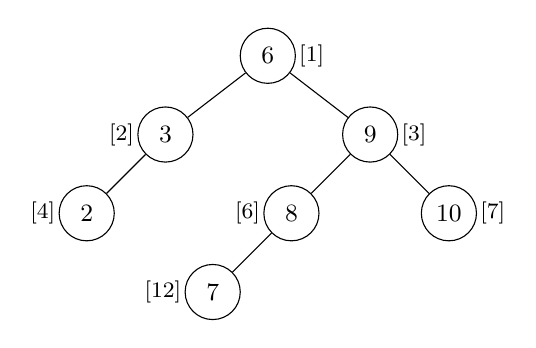
\begin{tikzpicture}[v/.style={circle,draw,minimum size=7mm,inner sep=0pt,font=\small},
    lb/.style={font=\footnotesize,inner sep=1pt}]
\node[v] (a) at (0,0) {6};
\node[v] (b) at (-1.3,-1) {3};
\node[v] (c) at (1.3,-1) {9};
\node[v] (d) at (-2.3,-2) {2};
\node[v] (e) at (0.3,-2) {8};
\node[v] (f) at (2.3,-2) {10};
\node[v] (g) at (-0.7,-3) {7};
\draw (a)--(b) (a)--(c) (b)--(d) (c)--(e) (c)--(f) (e)--(g);
\node[lb,right] at (a.east) {[1]};
\node[lb,left] at (b.west) {[2]};
\node[lb,right] at (c.east) {[3]};
\node[lb,left] at (d.west) {[4]};
\node[lb,left] at (e.west) {[6]};
\node[lb,right] at (f.east) {[7]};
\node[lb,left] at (g.west) {[12]};
\end{tikzpicture}
\end{center}
\begin{enumerate}[label=(\alph*)]
\item (5 points) Show postorder traversal of the above binary search tree.
\item (5 points) Please draw the resulting tree after inserting node 5 to the binary search tree above.
\item (10 points) Consider a binary search tree stored in array A and each node's key value is a
positive integer. For each tree node stored in A[$i$], its parent should be stored in A[$j$], where
$j=\lfloor i/2\rfloor$. For example, in the binary search tree above, the rightmost tree node
(i.e., node 10) is stored in A[7] and its parent should be stored in A[3] (i.e., node 9). Fill the
two blanks in the following procedure ``preorder'' (to complete a preorder traversal algorithm).
\begin{minted}[fontsize=\small,breaklines]{c}
void main() {
    int A[];

    For (i=1; ...; i++)
        A[i] = -1. /*initial value*/
    preorder(1);
}

void preorder(int i) {
    If A[i]<> -1 {
        printf("%d", A[i])
        preorder(__________);
        preorder(__________);}
}
\end{minted}
\end{enumerate}
\end{pastexam}

\begin{pastsoln}
答案：(a) $2, 3, 7, 8, 10, 9, 6$；(b) $5$ 成為 $3$ 的右子節點（存在 $A[5]$），圖在下面；
(c) 兩格依序填 \texttt{2*i} 和 \texttt{2*i+1}。

\textbf{(a)} 後序是「左子樹、右子樹、根」（資結書第~7.3~節，虛擬碼~7.1）。 根 $6$ 的左子樹是
$3(2)$，後序 $2, 3$；右子樹以 $9$ 為根：先走 $9$ 的左子樹 $8(7)$ 得 $7, 8$，再走右子樹 $10$，
最後 $9$，得 $7, 8, 10, 9$；最後是根 $6$。 合起來
\[
2,\ 3,\ 7,\ 8,\ 10,\ 9,\ 6 .
\]
這是二元搜尋樹，中序應該由小到大：$2, 3, 6, 7, 8, 9, 10$，可以拿來核對樹沒有讀錯。

\textbf{(b)} 照資結書第~9.2~節的插入（虛擬碼~9.6），從根往下比：$5 < 6$ 往左到 $3$；$5 > 3$ 往右，
$3$ 沒有右子節點，$5$ 就放在那裡，編號 $2 \cdot 2 + 1 = 5$。 其他節點都不動：
\begin{center}
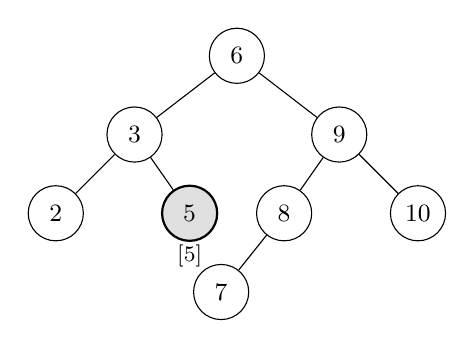
\begin{tikzpicture}[v/.style={circle,draw,minimum size=7mm,inner sep=0pt,font=\small},
    nv/.style={v,fill=black!12,line width=0.8pt},
    lb/.style={font=\footnotesize,inner sep=1pt}]
\node[v] (a) at (0,0) {6};
\node[v] (b) at (-1.3,-1) {3};
\node[v] (c) at (1.3,-1) {9};
\node[v] (d) at (-2.3,-2) {2};
\node[nv] (h) at (-0.6,-2) {5};
\node[v] (e) at (0.6,-2) {8};
\node[v] (f) at (2.3,-2) {10};
\node[v] (g) at (-0.2,-3) {7};
\draw (a)--(b) (a)--(c) (b)--(d) (b)--(h) (c)--(e) (c)--(f) (e)--(g);
\node[lb,below] at (h.south) {[5]};
\end{tikzpicture}
\end{center}

\textbf{(c)} 「$A[i]$ 的父節點在 $A[\lfloor i/2 \rfloor]$」反過來說，就是 $A[i]$ 的左子節點在
$A[2i]$、右子節點在 $A[2i+1]$（資結書第~7.2.1~節，編號從 $1$ 開始的那一欄）。 例如 $9$ 在 $A[3]$，
左子節點 $8$ 在 $A[6]$、右子節點 $10$ 在 $A[7]$。 前序是「根、左子樹、右子樹」，所以先印
$A[i]$，再走左子樹、再走右子樹：
\begin{center}
\texttt{preorder(2*i);}\qquad \texttt{preorder(2*i+1);}
\end{center}
沒有節點的格子是初值 $-1$（題目說鍵值都是正整數，所以 $-1$ 不會和真的鍵混淆），
\texttt{If A[i]<> -1} 不成立就直接返回，這就是遞迴的終止條件。 兩格的順序不能對調：
先 \texttt{2*i+1} 再 \texttt{2*i} 會變成「根、右、左」，不是前序。

要讓這支程式不讀到陣列外面，陣列要夠大：葉節點 $A[i]$ 也會呼叫 \texttt{preorder(2*i)} 和
\texttt{preorder(2*i+1)}，所以 $A$ 要開到最大編號的兩倍再加一，而且這些格子都要初始化成 $-1$。
題目的樹最大編號是 $12$，要用到 $A[25]$。

用原來的樹追蹤，印出的順序是 $6, 3, 2, 9, 8, 7, 10$（\texttt{"\%d"} 沒有分隔，實際印出來會黏在一起）；
插入 $5$ 之後是 $6, 3, 2, 5, 9, 8, 7, 10$。
\end{pastsoln}
